\chapter{ديناميكيات فريدمان: المادة، والإشعاع، وطاقة الفراغ}

\lectureoverview{يمكن صياغة حركيات الكون المتمدد في سطر واحد: تنمو المسافات الفيزيائية بعامل قياس \(a(t)\). والمشكلة الآن هي تحديد تلك الدالة. سنستعيد معادلة فريدمان للفضاء المستوي من حفظ الطاقة النيوتني، ونحلها أولًا للمادة العادية، ثم نرى لماذا يقود كل من الإشعاع وطاقة الفراغ إلى تواريخ كونية مختلفة تمامًا.}

\section{الهندسة المطلوب تفسيرها}

عند زمن كوني ثابت، يبدو الكون على المقاييس الكبيرة متجانسًا ومتساوي الخواص. فالمجرات والعناقيد والحشود العظمى سمات حقيقية بلا شك، لكن على مقاييس مئات الملايين أو مليارات السنين الضوئية يصبح توزعها منتظمًا على نحو لافت. وتسمى هذه الانتظامية التجريبية بالمبدأ الكوني. والاسم لا يجعله مبرهنة؛ فقوة هذا المبدأ تأتي من الرصد.

هناك حقيقة تجريبية ثانية. ضمن حدود الدقة الحالية، تتصرف المثلثات المكانية الكبيرة كمثلثات إقليدية. والمقارنة بمسح ملعب كرة قدم مفيدة. فإذا كوَّنت خطوط مشدودة بإحكام مثلثاتٍ يكون مجموع زواياها \(180^\circ\)، فهذا لا يثبت أن الأرض مستوية على المستوى الكلي. وإنما يبيّن أن نصف قطر انحناء الأرض كبير مقارنة بالملعب. وللمسح الكوني الصورة المنطقية نفسها: فقد يكون للفضاء نصف قطر انحناء كبير جدًا، لكنه يُقارب جيدًا كمستوٍ على امتداد المنطقة القابلة للرصد.

الهندسة المرجعية هي زمكان مينكوفسكي،
\begin{equation}
  d\tau^2=dt^2-\left(dx^2+dy^2+dz^2\right).
  \label{eq:l09-minkowski}
\end{equation}
والتعبير بين القوسين ليس إلا عنصر المسافة الإقليدية في ثلاثة أبعاد. أمّا في النسبية العامة، فعلى النقيض من ذلك، فإن معاملات تفاضلات الإحداثيات هي حقول. وقد تتغير مع الموضع والزمن، وقد تظهر أيضًا حدود مختلطة. وهذه المعاملات المترية هي النظائر النسبية لحقل الجاذبية النيوتني.

\begin{figure}[H]
  \centering
  \includegraphics[width=0.72\textwidth]{lecture_09_figure_01.png}
  \caption{عنصر الزمن الخاص في مينكوفسكي كما كُتب في بداية المحاضرة. إطار المصدر عند 00:01:50.}
  \label{fig:l09-minkowski-board}
\end{figure}

في كون متمدد مستوٍ مكانيًا، لا يترك التجانس وتساوي الخواص إلا عامل قياس واحدًا تابعًا للزمن:
\begin{equation}
  d\tau^2=dt^2-a^2(t)\left(dx^2+dy^2+dz^2\right).
  \label{eq:l09-flat-frw}
\end{equation}
نستخدم وحدات يكون فيها \(c=1\)، لذا يكون للزمن والطول الأبعاد نفسها. وهناك اصطلاحان متسقان. يمكن إعطاء \(x,y,z\) أبعاد الطول واعتبار \(a\) بلا أبعاد، أو معاملة \(x,y,z\) على أنها وسوم بلا أبعاد وترك \(a\) يحمل أبعاد الطول. وتستعمل المحاضرة الاصطلاح الثاني لأنه يُظهر المعنى الفيزيائي لـ \(a(t)\).

\begin{figure}[H]
  \centering
  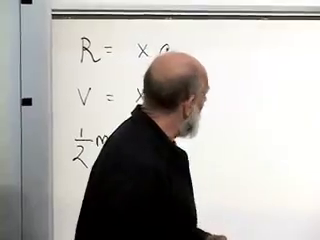
\includegraphics[width=0.72\textwidth]{lecture_09_figure_02.png}
  \caption{المترية المستوية المتمددّة، حيث يضرب عامل القياس عنصر الخط المكاني الإقليدي. إطار المصدر عند 00:09:12.}
  \label{fig:l09-expanding-metric-board}
\end{figure}

تخيل إحداثيات مرسومة على صفيحة مطاطية. تبقى علامات الإحداثيات مثبتة على الصفيحة بينما تنمو المسافة الفيزيائية بينها. وهكذا فإن فرقًا إحداثيًا مثل «من \(x=0\) إلى \(x=1\)» ليس إلا زوجًا من الوسوم. والمسافة التي يمثلها ذلك الفاصل هي \(a(t)\). ومسألة إيجاد المعادلة التي تحكم عامل القياس هذا هي المسألة الديناميكية في المحاضرة.

\section{الهندسات المكانية المغلقة والمستوية والمفتوحة}

الاستواء تبسيط رصدي، وليس نتيجة للتجانس. وهناك ثلاث هندسات مكانية متجانسة ومتساوية الخواص: ذات انحناء موجب، وصِفري، وسالب. ولفهم الحالة ذات الانحناء الموجب، يفيد أن نكون دقيقين بشأن البعد.

المكان الهندسي
\begin{equation}
  X_1^2+X_2^2=R^2
\end{equation}
هو دائرة، أي كرة أحادية \(S^1\). وداخلها الممتلئ قرص، ويُسمى أيضًا كرة ثنائية. وبإضافة إحداثي تضمين واحد نحصل على
\begin{equation}
  X_1^2+X_2^2+X_3^2=R^2,
\end{equation}
وهي الكرة الثنائية العادية \(S^2\). وبإضافة إحداثي تضمين رابع نحصل على
\begin{equation}
  X_1^2+X_2^2+X_3^2+X_4^2=R^2,
  \label{eq:l09-three-sphere}
\end{equation}
وهي كرة ثلاثية \(S^3\)، وهي نفسها فضاء ثلاثي الأبعاد. لا نستطيع تصور تضمينها رباعي الأبعاد، لكن الهندسة الجوهرية لا تحتاج إلى ذلك التضمين لكي توجد.

\begin{figure}[H]
  \centering
  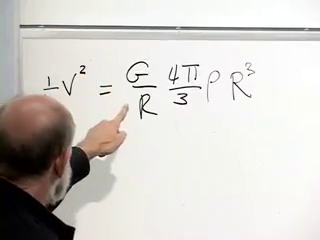
\includegraphics[width=0.72\textwidth]{lecture_09_figure_03.png}
  \caption{معادلة التضمين المستخدمة لتقديم الكرة الثلاثية. إطار المصدر عند 00:16:40.}
  \label{fig:l09-three-sphere-board}
\end{figure}

كل نقطة على كرة مثالية مكافئة هندسيًا لكل نقطة أخرى، وكل اتجاه عند نقطة ما مكافئ لأي اتجاه آخر. لذلك فالكرة متجانسة ومتساوية الخواص معًا. وإذا ضُرب نصف قطرها في \(a(t)\)، فإن الفضاء كله يتمدد أو ينكمش من دون تعيين مركز على الكرة. وإرجاع مثل هذا الكون إلى الماضي لا يضع كل المادة في موضع خاص واحد ضمن خلاء خارجي. بل إن الفضاء بأسره يصغر، فتغدو كل زوج من النقاط متقاربًا. والانفجار العظيم ليس انفجارًا من نقطة واحدة في الفضاء.

على كرة ذات انحناء موجب، يكون مجموع زوايا المثلثات الجيوديسية أكبر من \(180^\circ\). وفي المثلثات المستوية يكون مجموع الزوايا مساويًا تمامًا لـ \(180^\circ\). وفي هندسة متجانسة ذات انحناء سالب، تُمثَّل على نحو غير كامل بسطح سرجي، يكون مجموع الزوايا أقل من \(180^\circ\). وهذه الاختبارات الجوهرية تميّز بين الحالات الثلاث.

\begin{figure}[H]
  \centering
  \includegraphics[width=0.72\textwidth]{lecture_09_figure_07.png}
  \caption{الانحناء الموجب والصِفري والسالب موضحة عبر أشكالها المثلثية المميزة. إطار المصدر عند 00:37:30.}
  \label{fig:l09-curvature-board}
\end{figure}

إن متريةً محليةً مستويةً تمامًا لا تثبت بمفردها أن الفضاء غير منتهٍ طوبولوجيًا. فالطوبولوجيات المستوية المدمجة ممكنة رياضيًا، مع أن المحاضرة تعتمد أبسط نموذج إقليدي لا نهائي.
\editorialnote{هذا التحفظ المتعلق بالطوبولوجيا الشاملة غير مطلوب لأي من الديناميات المحلية اللاحقة.}

\section{الوسوم المواكبة للتمدد وقانون هابل}

لنعد الآن إلى الصفيحة المستوية المتمددة ونرسم عليها شبكة إحداثيات. في الإحداثيات المواكبة للتمدد، تتمدد الشبكة مع جريان المادة على المقاييس الكبيرة. وتحتفظ مجرة، أو على نحو أدق تجمّع من المجرات موصوف على نحو خشن بما يكفي، بوسم إحداثي ثابت تقريبًا، حتى مع تغيّر بعدها الفيزيائي عن جسم آخر مواكب للتمدد.

\begin{figure}[H]
  \centering
  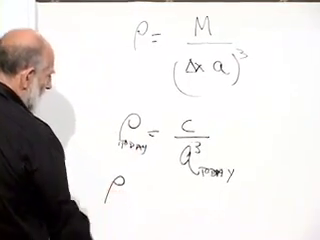
\includegraphics[width=0.72\textwidth]{lecture_09_figure_04.png}
  \caption{شبكة إحداثيات تُحمل مع صفيحة مكانية متمددة.
  إطار المصدر عند 00:22:20.}
  \label{fig:l09-comoving-grid-board}
\end{figure}

بالنسبة إلى جسمين يفصل بينهما على طول المحور \(x\) فاصل متواكب ثابت مقداره \(\Delta x\)، تكون المسافة الفيزيائية بينهما
\begin{equation}
  D(t)=a(t)\,\Delta x.
  \label{eq:l09-physical-distance}
\end{equation}
وباِشتقاق ذلك مع تثبيت \(\Delta x\) نحصل على
\begin{equation}
  v(t)=\dot a(t)\,\Delta x
      =\frac{\dot a(t)}{a(t)}D(t).
\end{equation}
وبتعريف
\begin{equation}
  H(t)\equiv\frac{\dot a(t)}{a(t)},
  \label{eq:l09-hubble-parameter}
\end{equation}
نحصل على قانون هابل،
\begin{equation}
  v=H(t)D.
  \label{eq:l09-hubble-law}
\end{equation}
إن كلمة «ثابت» في عبارة «ثابت هابل» تعني الثبات عبر الفضاء عند زمن كوني محدد. ولا تعني الثبات عبر التاريخ الكوني.

\begin{figure}[H]
  \centering
  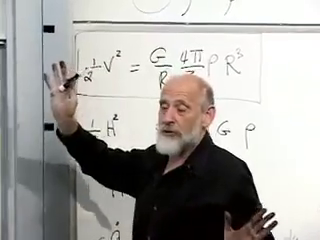
\includegraphics[width=0.72\textwidth]{lecture_09_figure_05.png}
  \caption{اشتقاق اللوح لـ \(D=a\Delta x\)،
  \(v=(\dot a/a)D=HD\). إطار المصدر عند 00:26:40.}
  \label{fig:l09-hubble-board}
\end{figure}

\begin{classroomqa}
\audiencequestion{إذا رأينا مجرة بعيدة كما كانت في زمن أبكر، فهل ينبغي حقًا أن يساوي معامل هابل المستنتج لها القيمة المقاسة في جوارنا اليوم؟}
\lecturerresponse{لا يكون ذلك إلا عندما يكون زمن النظر إلى الماضي صغيرًا مقارنة بعمر الكون. فعلى المسافات المعتدلة، يتغير \(H(t)\) تغيرًا طفيفًا بما يكفي لأن يكون عدد واحد مفيدًا. أمّا على المسافات الكونية حقًا، فإننا نرى حقبًا أبكر، ويجب تضمين الاعتماد الزمني لكل من \(a\) و\(H\). وذلك أحد الأسباب التي تجعلنا نحتاج إلى معادلة ديناميكية لعامل القياس.}
\end{classroomqa}

\section{الأشعة العدمية في نظام إحداثيات متمدد}

\begin{classroomqa}
\audiencequestion{هل يؤثر عامل القياس في انتشار الضوء بين المجرات البعيدة؟}
\lecturerresponse{يسلك شعاع الضوء مسارًا عدميًا، لذا \(d\tau=0\). وبالنسبة إلى شعاع يتحرك على طول المحور \(x\) الموجب، يكون \(dy=dz=0\)، وتعطي المترية المتمددة
\begin{align}
  0&=dt^2-a^2(t)dx^2,
  &dt&=a(t)dx,\notag\\
  &&\frac{dx}{dt}&=\frac{1}{a(t)}.
  \label{eq:l09-null-ray}
\end{align}
تتناقص السرعة الإحداثية كلما نما \(a(t)\)، لكن السرعة الفيزيائية المحلية للضوء تبقى \(c=1\). ويمثل فاصل إحداثي ثابت مسافة فيزيائية متزايدة.}
\end{classroomqa}

\begin{figure}[H]
  \centering
  \includegraphics[width=0.72\textwidth]{lecture_09_figure_06.png}
  \caption{الشرط العدمي و\(dt=a(t)dx\) لانتشار الضوء الشعاعي.
  إطار المصدر عند 00:30:54.}
  \label{fig:l09-null-board}
\end{figure}

يمكن اختيار إحداثيات يبدو فيها هذا الأمر نفسه بصيغة «يتباطأ الضوء كلما ازداد البعد»، لكن الأطوال والساعات تكتسب عندئذٍ أوصافًا مربكة بالمقدار المناظر. ولغة الفضاء المتمدد أنظف لأنها تحفظ العبارة المحلية القائلة إن كل راصد في سقوط حر يقيس السرعة نفسها للضوء.

\begin{classroomqa}
\audiencequestion{هل يوجد دليل على أن انتشار الضوء المحلي والفيزياء الذرية متماثلان في المجرات البعيدة؟}
\lecturerresponse{المقارنات اللابعدية وحدها ذات معنى إجرائي. اختر حجمًا ذريًا وحدةً للطول، وفترة ذرية أو نووية وحدةً للزمن، ثم اسأل كم عدد هذه الفترات الذي يحتاج إليه الضوء ليعبر الطول المختار. وتدعم الرصود الطيفية القول إن هذه النسب اللابعدية هي نفسها في المناطق البعيدة. والدليل غير مباشر، لكنه بالضبط نوع المقارنة الذي يُختبر به تماثل القوانين المحلية.}
\end{classroomqa}

عندما كان الكون المرصود صغيرًا للغاية، كان يمكن للضوء أن يعبر منطقة فيزيائية معيّنة بسرعة بحسب وحدة عبور الضوء الموافقة. وهذا لا يعني أن \(c\) كان مختلفًا. بل يعني أن المنطقة نفسها كانت صغيرة.

\section{كرة نيوتنية داخل الكون}

ننتقل الآن من الحركيات إلى الديناميكيات. لنضع أنفسنا عند الأصل ولنرسم كرة كبيرة بما يكفي لتحتوي كثيرًا من المجرات والعناقيد. اختر مجرة على حدّها. في كون متجانس يكون توزع الكتلة متناظرًا تناظرًا كرويًا حولنا، وتعطينا مبرهنة القشرة لنيوتن حقيقتين حاسمتين:
\begin{enumerate}
  \item كل مادة موزعة كرويًا خارج نصف القطر المختار تؤثر في المجرة الحدّية بقوة نيوتنية محصلة تساوي صفرًا؛
  \item كل المادة داخل الكرة تؤثر، في هذه الحركة الشعاعية، كما لو كانت متركزة في المركز.
\end{enumerate}
نستخدم إطارًا نكون فيه ساكنين، لذا تُقاس السرعات والتسارعات في الحجة التالية بالنسبة إلينا.

\begin{figure}[H]
  \centering
  \includegraphics[width=0.72\textwidth]{lecture_09_figure_08.png}
  \caption{بناء مبرهنة القشرة: نحن في المركز ومجرة اختبارية على حدّ كرة كبيرة متجانسة. إطار المصدر عند 00:41:10.}
  \label{fig:l09-shell-board}
\end{figure}

\begin{figure}[H]
  \centering
  \begin{tikzpicture}[scale=0.92,>=Latex]
    \draw[thick] (0,0) circle (2.35);
    \fill (0,0) circle (2pt) node[below left] {us};
    \fill (2.35,0) circle (2.2pt) node[right] {test galaxy \(m\)};
    \draw[->,thick,blue!65!black] (0.18,0) -- (2.15,0)
      node[midway,above] {\(R=a(t)x\)};
    \draw[->,thick,red!65!black] (2.35,0.12) -- (3.25,0.12)
      node[midway,above] {\(v=\dot a(t)x\)};
    \node[align=center,text width=7cm] at (0,-2.85)
      {outside shells cancel;\\enclosed mass acts at the center};
  \end{tikzpicture}
  \caption{إعادة بناء واضحة للبناء النيوتني.}
  \label{fig:l09-shell-clean}
\end{figure}

إذا كان للمجرة إحداثي مساير للتمدد ثابت هو \(x\)، فإن نصف قطرها الفيزيائي وسرعتها هما
\begin{equation}
  R(t)=x a(t),
  \qquad
  v(t)=x\dot a(t)=H(t)R(t).
  \label{eq:l09-radius-velocity}
\end{equation}
ولتكن \(M\) الكتلة المحصورة داخل الكرة و\(m\) كتلة مجرة الاختبار. عندئذ تكون الطاقة النيوتنية
\begin{equation}
  E=\frac12 m v^2-\frac{GMm}{R}.
  \label{eq:l09-newtonian-energy}
\end{equation}

\begin{figure}[H]
  \centering
  \includegraphics[width=0.72\textwidth]{lecture_09_figure_09.png}
  \caption{تسلسل اللوح الكامل لـ \(R=xa\) و\(v=x\dot a\)، ومعادلة الطاقة النيوتنية المخصَّصة للحالة \(E=0\). إطار المصدر عند 00:48:40.}
  \label{fig:l09-energy-board}
\end{figure}

قد تكون الطاقة موجبة أو صفرًا أو سالبة. لنبدأ عند الحد الفاصل بين الإفلات وإعادة الانهيار، \(E=0\)، الذي عنده
\begin{equation}
  \frac12 v^2=\frac{GM}{R}.
  \label{eq:l09-zero-energy}
\end{equation}

\begin{classroomqa}
\audiencequestion{ماذا تعني الطاقة الكلية الصفرية بالنسبة إلى المجرة المتباعدة؟}
\lecturerresponse{إنها بالضبط حالة سرعة الإفلات. فتعني الطاقة الموجبة حركة فوق سرعة الإفلات؛ وتعني الطاقة السالبة حركة دون سرعة الإفلات، وفي الصورة النيوتنية التي تحتوي على المادة فقط، عودة في نهاية المطاف. نبدأ عند الحد الفاصل بين هذين الاحتمالين، ثم نعود إلى الإشارتين الأخريين بعد اشتقاق معادلة الحالة المسطحة.}
\end{classroomqa}

\begin{classroomqa}
\audiencequestion{هل تتغير الكتلة المحصورة \(M\) مع تمدد الكرة؟}
\lecturerresponse{لا. الكرة مسايرة للتمدد، لذا تبقى الجسيمات نفسها داخلها. ينمو حجمها الفيزيائي وتنخفض كثافتها، لكن كتلتها الكلية المحصورة تبقى ثابتة. وهذا التمييز بين \(M\) و\(\rho(t)\) أساسي.}
\end{classroomqa}

لكثافة متجانسة \(\rho(t)\)،
\begin{equation}
  M=\frac{4\pi}{3}\rho(t)R^3.
  \label{eq:l09-enclosed-mass}
\end{equation}
وبالتعويض في \eqref{eq:l09-zero-energy} نحصل على
\begin{equation}
  \frac12 v^2
  =\frac{G}{R}\left(\frac{4\pi}{3}\rho R^3\right).
  \label{eq:l09-enclosed-energy}
\end{equation}

\begin{figure}[H]
  \centering
  \includegraphics[width=0.72\textwidth]{lecture_09_figure_10.png}
  \caption{تعويض الكتلة المحصورة في معادلة الطاقة الصفرية.
  إطار المصدر عند 00:54:16.060.}
  \label{fig:l09-enclosed-mass-board}
\end{figure}

باستخدام \(v=HR\)، نجد
\begin{align}
  \frac12 H^2R^2
    &=\frac{4\pi G}{3}\rho R^2,\\
  H^2
    &=\frac{8\pi G}{3}\rho.
\end{align}
ومن ثم فإن قانون التمدد للحالة ذات الطاقة الصفرية والمسطحة مكانيًا هو
\begin{equation}
  \boxed{\left(\frac{\dot a}{a}\right)^2
  =\frac{8\pi G}{3}\rho(t)}.
  \label{eq:l09-flat-friedmann}
\end{equation}
واختزال \(R^2\) ليس مصادفة. فلا بد لكون متجانس أن يعطي القيمة نفسها لـ \(H(t)\) أيًا كانت المجرة المسايرة للتمدد التي اختيرت بوصفها جسم الاختبار.

\begin{figure}[H]
  \centering
  \includegraphics[width=0.72\textwidth]{lecture_09_figure_11.png}
  \caption{اختزال نصف القطر وعلاقة فريدمان المسطحة الناتجة على اللوح. إطار المصدر عند 00:57:30.}
  \label{fig:l09-friedmann-board}
\end{figure}

\begin{classroomqa}
\audiencequestion{هل توجد أدلة على علاقة الطاقة الصفرية؟}
\lecturerresponse{يمكن استنتاج كلا الطرفين رصديًا: \(H\) من بيانات التباعد و\(\rho\) باحتساب النجوم والغاز والمادة المظلمة وطاقة الفراغ. وقد وجد القياس في زمن هذه المحاضرة أن الطرفين متسقان بدقة تقارب نسبة مئوية. وهذا القيد مهم: إذ يجب تضمين جميع أشكال الطاقة، كما أن مناقشة طاقة الفراغ اللاحقة تغيّر التأويل الساذج القائم على سرعة الإفلات.}
\end{classroomqa}

في الوحدات \(c=1\)، تكون لكثافة الكتلة وكثافة الطاقة الوحدات نفسها. ولذلك سيرمز الرمز \(\rho\) إلى كثافة الطاقة الكلية الملائمة للمكوّن الجاري بحثه.

\section{المادة العادية وقانون الثلثين}

لا تكون المعادلة \eqref{eq:l09-flat-friedmann} مغلقةً حتى نعرف كيف تتغير \(\rho(t)\). فلنملأ أولًا صندوقًا مستطيلًا مسايرًا للتمدد بجسيمات بطيئة الحركة وغير نسبية. أبعاده الإحداثية ثابتة، بينما ينمو حجمه الفيزيائي وفق
\begin{equation}
  V(t)=a^3(t)\,\Delta x\,\Delta y\,\Delta z.
\end{equation}
ويبقى عدد الجسيمات وكتلة السكون الكلية في الصندوق ثابتين، لذا
\begin{equation}
  \rho_{\mathrm m}(t)=\frac{C_{\mathrm m}}{a^3(t)}.
  \label{eq:l09-matter-dilution}
\end{equation}
وبالتطبيع إلى الحقبة الحالية \(t_0\)،
\begin{equation}
  \frac{\rho_{\mathrm m}(t)}{\rho_{\mathrm m,0}}
  =\left(\frac{a_0}{a(t)}\right)^3.
  \label{eq:l09-matter-normalized}
\end{equation}

\begin{figure}[H]
  \centering
  \includegraphics[width=0.72\textwidth]{lecture_09_figure_12.png}
  \caption{كثافة المادة، وتخففها وفق \(a^{-3}\)، وتطبيعها إلى القيمة الحالية. إطار المصدر عند 01:04:47.940.}
  \label{fig:l09-density-board}
\end{figure}

\begin{classroomqa}
\audiencequestion{ما القيمة التقريبية الحالية لكثافة طاقة الكون، وهل تستطيع الذرات العادية وحدها أن توفرها؟}
\lecturerresponse{إن إحصاء المادة الباريونية المرئية لا يعطي إلا جزءًا من الجواب. فلا بد أيضًا من تمثيل المادة المظلمة والطاقة المظلمة على هيئة كتلة-طاقة مكافئة. وتذكر المحاضرة مقياسًا تقريبيًا يتراوح من ذرة واحدة إلى بضع عشرات من مكافئات كتلة الهيدروجين في كل متر مكعب، مع التأكيد على رتبة المقدار لا على جرد دقيق.}
\end{classroomqa}

أدخل \eqref{eq:l09-matter-dilution} في
\eqref{eq:l09-flat-friedmann} واجمع جميع العوامل المستقلة عن الزمن في ثابت موجب \(C\):
\begin{equation}
  \left(\frac{\dot a}{a}\right)^2=\frac{C}{a^3},
  \qquad
  \dot a^2=\frac{C}{a}.
  \label{eq:l09-matter-ode}
\end{equation}
وهناك طريقتان واضحتان لحلها. إن تجربة حل بقانون قوى
\(a=K t^p\) تقتضي
\begin{equation}
  p-1=-\frac{p}{2},
  \qquad p=\frac23.
\end{equation}
وبصورة مكافئة، خذ فرع الجذر التربيعي الموافق للتمدد وأجرِ التكامل:
\begin{equation}
  a^{1/2}\frac{da}{dt}=\sqrt C,
  \qquad
  \int a^{1/2}da=\sqrt C\int dt,
\end{equation}
ومن ثم، بعد اختيار الانفجار العظيم مبدأً للزمن،
\begin{equation}
  a^{3/2}\propto t,
  \qquad
  \boxed{a(t)\propto t^{2/3}}.
  \label{eq:l09-matter-solution}
\end{equation}
يفقد الاشتقاق المباشر عاملًا لفترة وجيزة أثناء مطابقة المعاملات، ثم يعود إلى التكامل ويتحقق من الأسّ. وتُبقي الملاحظات على هذا التحقق، لكنها تعرض الجبر المصحح فقط.

\begin{figure}[H]
  \centering
  \includegraphics[width=0.72\textwidth]{lecture_09_figure_13.png}
  \caption{محاولة قانون القوى والأسّ المؤطَّر \(p=2/3\). إطار المصدر
  عند 01:13:05.}
  \label{fig:l09-matter-solution-board}
\end{figure}

باشتقاق الحل نحصل على
\begin{equation}
  H(t)=\frac{\dot a}{a}=\frac{2}{3t}.
  \label{eq:l09-matter-hubble}
\end{equation}
وكان معامل هابل أكبر في الماضي. ولذلك، عند النظر إلى مسافات بعيدة بما يكفي بحيث نرى زمنًا معتبرًا للنظر إلى الماضي، لا ينبغي تمديد العلاقة الخطية المحلية باستخدام \(H_0\) الحالي من دون تغيير.

\begin{figure}[H]
  \centering
  \includegraphics[width=0.72\textwidth]{lecture_09_figure_14.png}
  \caption{حساب \(\dot a/a\) عندما يكون \(a\propto t^{2/3}\) يعطي
  \(H=2/(3t)\). إطار المصدر عند 01:20:42.}
  \label{fig:l09-hubble-time-board}
\end{figure}

\section{إشارة الطاقة والانحناء المكاني}

قادنا الاستدلال النيوتني إلى الحالة المسطحة ذات الطاقة الصفرية. وتضيف النسبية العامة حقيقة لا يمكن الحصول عليها من مبرهنة القشرة وحدها: فإشارة الطاقة النوعية على النمط النيوتني تقابل إشارة الانحناء المكاني.
\begin{center}
\begin{tabular}{@{}>{\raggedright\arraybackslash}p{0.20\linewidth}
                    >{\raggedright\arraybackslash}p{0.29\linewidth}
                    >{\raggedright\arraybackslash}p{0.37\linewidth}@{}}
  \toprule
  الطاقة الكلية & الانحناء المكاني & المصير في نموذج المادة فقط \\
  \midrule
  موجبة & سالب (مفتوح) & يتمدد إلى الأبد \\
  صفرية & صفري (مسطّح) & يقترب من حد الإفلات \\
  سالبة & موجب (مغلق) & يتمدد، ثم ينعطف، ثم ينهار من جديد \\
  \bottomrule
\end{tabular}
\end{center}
ويفترض العمود الأخير عدم وجود طاقة فراغ. وفي تشبيه المقذوفات، تعني الطاقة الموجبة أن الحركة فوق سرعة الإفلات، وتعني الطاقة الصفرية أنها عند سرعة الإفلات تمامًا، وتعني الطاقة السالبة أنها دون سرعة الإفلات. وتطابق معادلات أينشتاين هذه الحالات الثلاث مع الهندسة المكانية المفتوحة والمسطحة والمغلقة، على الترتيب.

\section{الفوتونات وقانون النصف}

يفترض قانون المادة \(\rho\propto a^{-3}\) أن طاقة كل جسيم ثابتة تقريبًا بينما تنخفض الكثافة العددية. وتخالف الفوتونات هذا الافتراض. فبالنسبة إلى فوتون،
\begin{equation}
  E=h\nu=\frac{hc}{\lambda}.
\end{equation}
يمدّ التمدد طول موجته بنسبة تتناسب مع عامل القياس،
\begin{equation}
  \lambda\propto a,
  \qquad E\propto a^{-1}.
\end{equation}
ولا تزال الكثافة العددية للفوتونات تنخفض كما \(a^{-3}\)، وتضيف طاقة كل فوتون عاملًا إضافيًا مقداره \(a^{-1}\). لذلك
\begin{equation}
  \boxed{\rho_{\mathrm r}(t)\propto a^{-4}(t)}.
  \label{eq:l09-radiation-dilution}
\end{equation}

يجسد تشبيه وتر الغيتار الصورة الفيزيائية. انقر وترًا ثم أطِل جزأه المهتز: يزداد الطول الموجي وتنخفض النغمة. ويتصرف نمط فوتوني في صندوق مساير للتمدد آخذ في التوسع على نحو مشابه. وإذا عكسنا الصورة، فإن الانضغاط يقصر الأطوال الموجية ويرفع طاقات الفوتونات.

\begin{figure}[H]
  \centering
  \includegraphics[width=0.72\textwidth]{lecture_09_figure_15.png}
  \caption{علاقة كثافة المادة بعد تمديدها على اللوح لتشمل قانون تحجيم الإشعاع \(\rho_{\mathrm r}\propto a^{-4}\). إطار المصدر عند 01:29:20.}
  \label{fig:l09-radiation-board}
\end{figure}

يؤدي استخدام \(\rho_{\mathrm r}\propto a^{-4}\) في معادلة فريدمان المستوية إلى
\begin{equation}
  \left(\frac{\dot a}{a}\right)^2=\frac{C_{\mathrm r}}{a^4},
  \qquad
  \dot a\propto a^{-1},
\end{equation}
ومن ثم
\begin{equation}
  \boxed{a(t)\propto t^{1/2}}.
  \label{eq:l09-radiation-solution}
\end{equation}
وهذا ينمو أبطأ من \(t^{2/3}\). وإذا عدنا بعيدًا بما يكفي إلى الماضي، فلا بد أن يهيمن الإشعاع على المادة العادية لأن \(a^{-4}\) يزداد أسرع من \(a^{-3}\) كلما تناقص \(a\). وتضع المحاضرة مرحلة تعادل المادة والإشعاع تقريبًا عند الحقبة التي كان فيها عامل القياس أصغر بنحو ألف مرة مما هو عليه اليوم. وقبل تلك المرحلة كان الكون خاضعًا لهيمنة الإشعاع؛ وبعدها كان، طوال فترة طويلة، خاضعًا لهيمنة المادة.

\section{طاقة الفراغ والتمدد الأسي}

لطاقة الفراغ سلوك معاكس فيما يتعلق بالاعتماد على عامل القياس. فكثافتها خاصية للفضاء الخالي، ولا تتناقص مع تمدد الكون:
\begin{equation}
  \rho_\Lambda=\text{constant}.
  \label{eq:l09-vacuum-density}
\end{equation}
وتصبح المادة العادية والإشعاع أكثف كلما اتجهنا نحو الماضي، بينما لا ينطبق ذلك على هذا الحد. ولذلك كانت أقل أهمية في الكون المبكر، وتصبح أكثر أهمية كلما تخلخلت المكونات الأخرى. وتستعمل المحاضرة التقدير السائد آنذاك، ومفاده أن طاقة الفراغ تسهم بنحو \(70\%\) من كثافة الطاقة الكونية اليوم.

مع ثبات \(\rho_\Lambda\)، تعطي المعادلة \eqref{eq:l09-flat-friedmann} معدل تمدد ثابتًا
\begin{equation}
  H_\Lambda=\sqrt{\frac{8\pi G}{3}\rho_\Lambda},
  \qquad
  \frac{\dot a}{a}=H_\Lambda.
\end{equation}
ولذلك
\begin{equation}
  \boxed{a(t)=a(t_i)e^{H_\Lambda(t-t_i)}}.
  \label{eq:l09-vacuum-solution}
\end{equation}

\begin{figure}[H]
  \centering
  \includegraphics[width=0.72\textwidth]{lecture_09_figure_16.png}
  \caption{معادلة الكثافة الثابتة التي تؤدي إلى تمدد أسي.
  إطار المصدر عند 01:35:48.}
  \label{fig:l09-vacuum-board}
\end{figure}

على المقياس المرصود المذكور في المحاضرة، يتضاعف البعد الخطي للكون خلال نحو عشرة إلى اثني عشر مليار سنة. ولا يزال أصل كثافة الفراغ الصغيرة هذه، ولكن غير المنعدمة، غير مفسَّر؛ أما وجودها وتأثيرها في التمدد فهما حقيقتان تجريبيتان.

\begin{classroomqa}
\audiencequestion{هل طاقة الفراغ هي نفسها الطاقة المظلمة في هذا النقاش؟}
\lecturerresponse{نعم. تدل «الطاقة المظلمة» هنا على كثافة ثابتة لطاقة الفراغ، أي ما يكافئ ثابتًا كونيًا. ويمكن تصوّر نماذج أكثر عمومية للطاقة المظلمة تعتمد على الزمن، لكنها ليست جزءًا من حساب هذه المحاضرة.}
\end{classroomqa}

\section{كيف يسبّب الكون المتمدد انزياح الضوء نحو الأحمر}

\begin{classroomqa}
\audiencequestion{كيف يمكن للفوتونات أن تعرف أننا اخترنا إحداثيات مسايرة للتمدّد، ومن ثم تخفض طاقتها؟}
\lecturerresponse{هي لا تستجيب لتسمياتنا. بل تنتشر خلال هندسة تتغير فيها المسافات الفيزيائية. والقطار الموجي الذي يشغل منطقة يتضاعف حجمها الفيزيائي يكتسب طولًا موجيًا متضاعفًا. أما الإحداثيات المسايرة فمجرد وسيلة تصف هذا التمطط بصورة مقتصدة؛ وهي لا تسببه.}
\end{classroomqa}

\begin{classroomqa}
\audiencequestion{من أين تأتي فوتونات الخلفية التي تصل إلينا اليوم؟}
\lecturerresponse{إن النظر إلى مسافات أبعد يعني النظر إلى أزمنة أبكر. وفي نهاية المطاف نرى الحقبة التي كانت فيها مادة الكون بلازما متأينة، معتمة لأن الفوتونات كانت تتبعثر مرارًا عن الجسيمات الحرة المشحونة. ويظهر الحد الذي استطاعت الفوتونات بعده أن تسافر إلينا بحرية للمرة الأخيرة على هيئة كرة تحيط بالراصد: سطح التبعثر الأخير.}
\end{classroomqa}

\begin{figure}[H]
  \centering
  \includegraphics[width=0.72\textwidth]{lecture_09_figure_17.png}
  \caption{الرسم التخطيطي المتمركز على الراصد لسطح التبعثر الأخير والأغلفة المتزايدة بُعدًا.
  إطار المصدر عند 01:42:05.}
  \label{fig:l09-last-scattering-board}
\end{figure}

\begin{figure}[H]
  \centering
  \begin{tikzpicture}[scale=0.9,>=Latex]
    \fill (0,0) circle (2pt) node[below] {observer};
    \draw[thick,orange!70!black] (0,0) circle (2.55);
    \node[orange!70!black,align=center] at (0,3.05)
      {surface of last scattering};
    \foreach \a in {25,75,145,210,285,335}{
      \draw[->,blue!60!black] ({2.55*cos(\a)},{2.55*sin(\a)}) --
        ({1.7*cos(\a)},{1.7*sin(\a)});
    }
    \draw[decorate,decoration={snake,amplitude=1.5pt,segment length=7pt},
      red!65!black,thick,->] (-2.5,0) -- (-0.15,0);
    \node[red!65!black,below] at (-1.35,-0.15)
      {redshifted photon};
  \end{tikzpicture}
  \caption{إعادة بناء منقّحة لصورة التبعثر الأخير.}
  \label{fig:l09-last-scattering-clean}
\end{figure}

انبعث الإشعاع بطيف مميز لبلازما حارة، ويصل إلينا بأطوال موجية أطول بنحو ألف مرة. وبلغة دوبلر المستعملة في المحاضرة، يبتعد السطح الباعث البعيد بسرعة، ويكون إشعاعه منزاحًا بشدة نحو الأحمر. وباللغة الهندسية، تُمطّ الموجة أثناء انتشارها. وكلتا الصورتين تعبّران عن العلاقة نفسها،
\begin{equation}
  1+z=\frac{\lambda_0}{\lambda_{\mathrm{em}}}
      =\frac{a_0}{a_{\mathrm{em}}}.
  \label{eq:l09-cosmological-redshift}
\end{equation}
\editorialnote{تمثل المعادلة \eqref{eq:l09-cosmological-redshift} الصيغة الكمية المعيارية لوصفي الاستطالة ودوبلر في المحاضرة.}

في حقبة رصد أبكر، لكانت كرة التبعثر الأخير أقرب في الصورة المناظرة، ولكانت فوتونات الخلفية المرصودة أقل انزياحًا نحو الأحمر، ومن ثم أعلى طاقة. ومع تقدم الزمن الكوني، تكون للفوتونات التي تصل إلى راصد مساير للتمدّد من تلك البلازما المبكرة أطوال موجية تزداد طولًا تدريجيًا.

\section{إلى أين تذهب طاقة الفوتون المنزاح نحو الأحمر؟}

\begin{classroomqa}
\audiencequestion{يُصدر فوتون بطاقة \(h\nu_{\mathrm{em}}\) ثم يصل منزاحًا نحو الأحمر بطاقة أقل. ماذا حدث للفارق؟}
\lecturerresponse{بدأ الاشتقاق النيوتني في الأصل بوصفه معادلة طاقة. وصيغته الكونية تربط معدل التمدد بكثافة طاقة المحتوى المادي، لذلك لا يمكن التعامل مع طاقة المادة والتمدد على أنهما حسابان محفوظان على نحو منفصل. وتصف المحاضرة طاقة الفوتون المفقودة بأنها تدخل في المحاسبة الحركية للتمدد. ويجعل تشبيه مكبس مملوء بالإشعاع ذلك محسوسًا: فضغط الإشعاع يدفع المكبس إلى الخارج، وتزداد الأطوال الموجية للفوتونات، وتصبح طاقتها المفقودة شغلًا ميكانيكيًا وطاقة حركية للمكبس.}
\end{classroomqa}

\begin{figure}[H]
  \centering
  \includegraphics[width=0.72\textwidth]{lecture_09_figure_18.png}
  \caption{تُظهر اللوحة معادلة الطاقة النيوتنية المؤطَّرة فوق معادلة فريدمان المناظرة.
  إطار المصدر عند 01:44:42.}
  \label{fig:l09-energy-bookkeeping-board}
\end{figure}

\begin{classroomqa}
\audiencequestion{ما الذي يربط طاقة الإشعاع بالتمدد؟}
\lecturerresponse{الضغط. ففي أسطوانة ذات مكبس متحرك، تنقل الفوتونات زخمًا إلى الجدار. ومع تحرك المكبس، يبذل الإشعاع شغلًا؛ فتزداد أطوالها الموجية وتنخفض طاقتها. وليس في الكون المتجانس المتمدد مكبس خارجي حرفي، لكن تشبيه \(p\,dV\) يوضح لماذا تنخفض كثافة طاقة الإشعاع أسرع مما يفسره تخفف العدد وحده.}
\end{classroomqa}

\begin{figure}[H]
  \centering
  \includegraphics[width=0.72\textwidth]{lecture_09_figure_19.png}
  \caption{المكبس المتحرك المملوء بالفوتونات والمستخدَم لتصوير شغل الضغط.
  إطار المصدر عند 01:46:40.}
  \label{fig:l09-piston-board}
\end{figure}

\begin{figure}[H]
  \centering
  \begin{tikzpicture}[scale=0.92,>=Latex]
    \draw[thick] (0,0) rectangle (5.3,2.6);
    \draw[very thick] (4.25,0) -- (4.25,2.6);
    \draw[very thick] (4.25,1.3) -- (5.25,1.3);
    \draw[->,thick,red!65!black] (5.25,1.3) -- (6.2,1.3)
      node[right] {moving piston};
    \foreach \y in {0.55,1.3,2.05}{
      \draw[decorate,decoration={snake,amplitude=1.4pt,segment length=6pt},
        blue!65!black,->] (0.35,\y) -- (3.9,\y);
    }
    \node at (2.15,-0.45) {radiation does \(p\,dV\) work};
  \end{tikzpicture}
  \caption{إعادة بناء منقّحة لتشبيه الإشعاع والمكبس.}
  \label{fig:l09-piston-clean}
\end{figure}

تتطلب الطاقة في النسبية العامة قدرًا من الحذر. ففي زمكان متمدد عام، قد لا توجد طاقة كلية محفوظة وحيدة مماثلة لطاقة نظام نيوتني معزول. ومع ذلك يبقى انحفاظ موتر الإجهاد-الطاقة موضعيًا ساريًا، وبالنسبة إلى مائع متجانس فإنه يعطي معادلة الاستمرارية
\begin{equation}
  \dot\rho+3H(\rho+p)=0,
  \label{eq:l09-continuity}
\end{equation}
التي تتضمن حد شغل الضغط الكامن وراء قوانين تدرج المادة والإشعاع.\editorialnote{تمثل المعادلة \eqref{eq:l09-continuity} الصياغة الموضعية الدقيقة في النسبية العامة التي تقوم عليها محاكاة المحاضرة المتعمدة للمحاسبة النيوتنية للطاقة.}

تجعل طاقة الفراغ هذا اللغز أشد حدة على نحو خاص. فبما أن كثافتها تبقى ثابتة بينما يزداد الحجم، فإن طاقة الفراغ الكلية في منطقة مسايرة للتمدّد تزداد. وضغطها السالب جزء من المصدر الثقالي، وهو يدفع التمدد المتسارع. لذلك لا ينبغي المطالبة بانحفاظ منفصل لما يُسمى بسذاجة «طاقة المادة في صندوق مساير للتمدّد» من دون إدخال الهندسة وشغل الضغط.

\section{لماذا يمكن إزالة عامل القياس من الحد الزمني}

\begin{classroomqa}
\audiencequestion{لماذا يضرب عامل القياس الجزء المكاني من المترية لا الجزء الزمني؟}
\lecturerresponse{ذلك اختيار لإحداثي الزمن. افترض أننا نبدأ بإحداثي الزمن المطابق \(t\) بحيث
\begin{equation}
  d\tau^2=A^2(t)\left(dt^2-dx^2\right).
\end{equation}
وعرّف زمنًا كونيًا جديدًا \(T\) بالعلاقة
\begin{equation}
  dT=A(t)\,dt.
\end{equation}
فعندئذ
\begin{equation}
  d\tau^2=dT^2-A^2\bigl(t(T)\bigr)dx^2.
\end{equation}
يكون العامل المشترك أمام تفاضل الزمن قد اختفى، بينما يبقى عامل القياس الفيزيائي في الحد المكاني.}
\end{classroomqa}

\begin{figure}[H]
  \centering
  \includegraphics[width=0.72\textwidth]{lecture_09_figure_20.png}
  \caption{إعادة تعريف الزمن \(dT=A(t)dt\) التي تحوّل الزمن المطابق إلى زمن كوني.
  إطار المصدر عند 01:51:05.}
  \label{fig:l09-time-reparam-board}
\end{figure}

\section{الانحناء وطاقة الفراغ والمصير الكوني}

\begin{classroomqa}
\audiencequestion{إذا كان الكون ذا انحناء موجب، أفلا ينبغي أن نرى المجرات آتية نحونا بالفعل؟}
\lecturerresponse{ليس بالضرورة. فالمقذوف الذي يُطلَق بسرعة دون سرعة الإفلات يسير أولًا إلى الخارج، ويبلغ نقطة انقلاب، ثم لا يعود ساقطًا إلا لاحقًا. ونحن نرصد الكون خلال طور تمدد. ومن دون طاقة فراغ، فإن كونًا ماديًا ذا انحناء موجب سينكمش من جديد في نهاية المطاف. أما طاقة فراغ موجبة وكبيرة بما يكفي فتمنع ذلك الانعطاف، وتبدو القيمة المرصودة كبيرة بما يكفي لجعل التمدد الطويل الأمد أسيًا بصرف النظر عن انحناء مكاني صغير.}
\end{classroomqa}

ليس المستقبل الأسي فردوسًا طاقيًا. فالنجوم تنطفئ في نهاية المطاف، وتنخفض كثافتا المادة والإشعاع أسيًا، وتنتقل المناطق البعيدة إلى ما وراء الاتصال السببي. وتبقى طاقة الفراغ، بينما تصبح البنى العادية أبرد تدريجيًا وأكثر تخلخلًا.

\begin{classroomqa}
\audiencequestion{إذا عدنا أبعد إلى الماضي، فهل يكون عدد الفوتونات أكبر من عدد الجسيمات العادية؟}
\lecturerresponse{إن نسبة عدد الفوتونات إلى عدد الباريونات هائلة بالفعل، وتقارب \(10^{10}\) فوتونًا لكل باريون في تقدير المحاضرة، ويظل كلٌّ منهما، ضمن حجم مواكب للتمدد، ثابتًا تقريبًا. وما يتغير كلما اتجهنا نحو الماضي هو أساسًا الطاقة لكل فوتون. وترتفع طاقات الفوتونات على نحو \(a^{-1}\)، في حين أن كتل السكون غير النسبية لا تزداد. لذلك يهيمن الإشعاع على كثافة الطاقة في الأزمنة المبكرة، مع أن نسبة العدد نفسها لا يلزم أن تتغير.}
\end{classroomqa}

الدرس المركزي هو أن الهندسة وحدها لا تحدد التاريخ الكوني. فمعادلة فريدمان المسطحة توفّر العلاقة بين التمدد وكثافة الطاقة، لكن المحتوى المادي هو الذي يحدد الاعتماد على الزمن. فالمادة غير النسبية تعطي \(a\propto t^{2/3}\)، والإشعاع يعطي \(a\propto t^{1/2}\)، وطاقة الفراغ الثابتة تعطي تمددًا أسيًا. وهذه القوانين الثلاثة تنظّم العصور المتعاقبة للكون وتفسّر لماذا يتحكم عامل القياس نفسه في المسافات، والانزياحات نحو الأحمر، ومعامل هابل المتغيّر.
